\chapter{Validation of the algorithm one- point stage}

The results from the previous parameter are showed at figure \ref{fig:Nodes_Paths_2wv_1deg_5s} shows that algorithm left a triangle shape just at the center and this angle range correspond to the \textit{no-go-zone}.  \par \noindent

The marks on green, only at one side of the start point, on figure \ref{fig:nodes_2wv_5deg_5s} are the nodes that meet the criteria about the angle and the \textit{no-go zone}. The other side was not plotted %in this way to avoid confusion 
since the \acrshort{vpp} is assumed symmetrical.% \par \noindent
From all these nodes, considering only the right side of the graph, 14 paths with the smallest time were plotted on figure \ref{fig:Paths_2wv_5deg_5s}, the top three paths (minimal time) were marked in blue and it shows that 2 of them have the same time but they were developed at different angles. The figure also shows that these paths do not bend after 1500 meters from the vertical axis, which is approx. 1.73 times the mid-distance between the two marks. %85\% of the total distance between the start point and the target point. \par \noindent

Although the number of nodes, none of them reach the target exactly, and the algorithm send a message about it, so the partial solutions were stored. Using the stored data and the some of the previous formulas the time were estimated figure \ref{fig:PathsZoom_2wv_5deg_5s} shows that they are at least 1.5 meter away from the target. The minimal time path from them is just below the target while the paths with the same time looks almost symmetrical with the same horizontal distance to the target, less than 6 meters. The total time of these two paths has an error about 15\% comparing with results of the first leg from the race 1 of the World Cup Series 2017 at Hyères, France, \cite{SAPsailingana}. \par   
 
\begin{figure} [hbt!]
  \centering
  \subfloat[Nodes using 1 attack with $\Delta t$ =5s and $\Delta \Psi =5\degree$.] {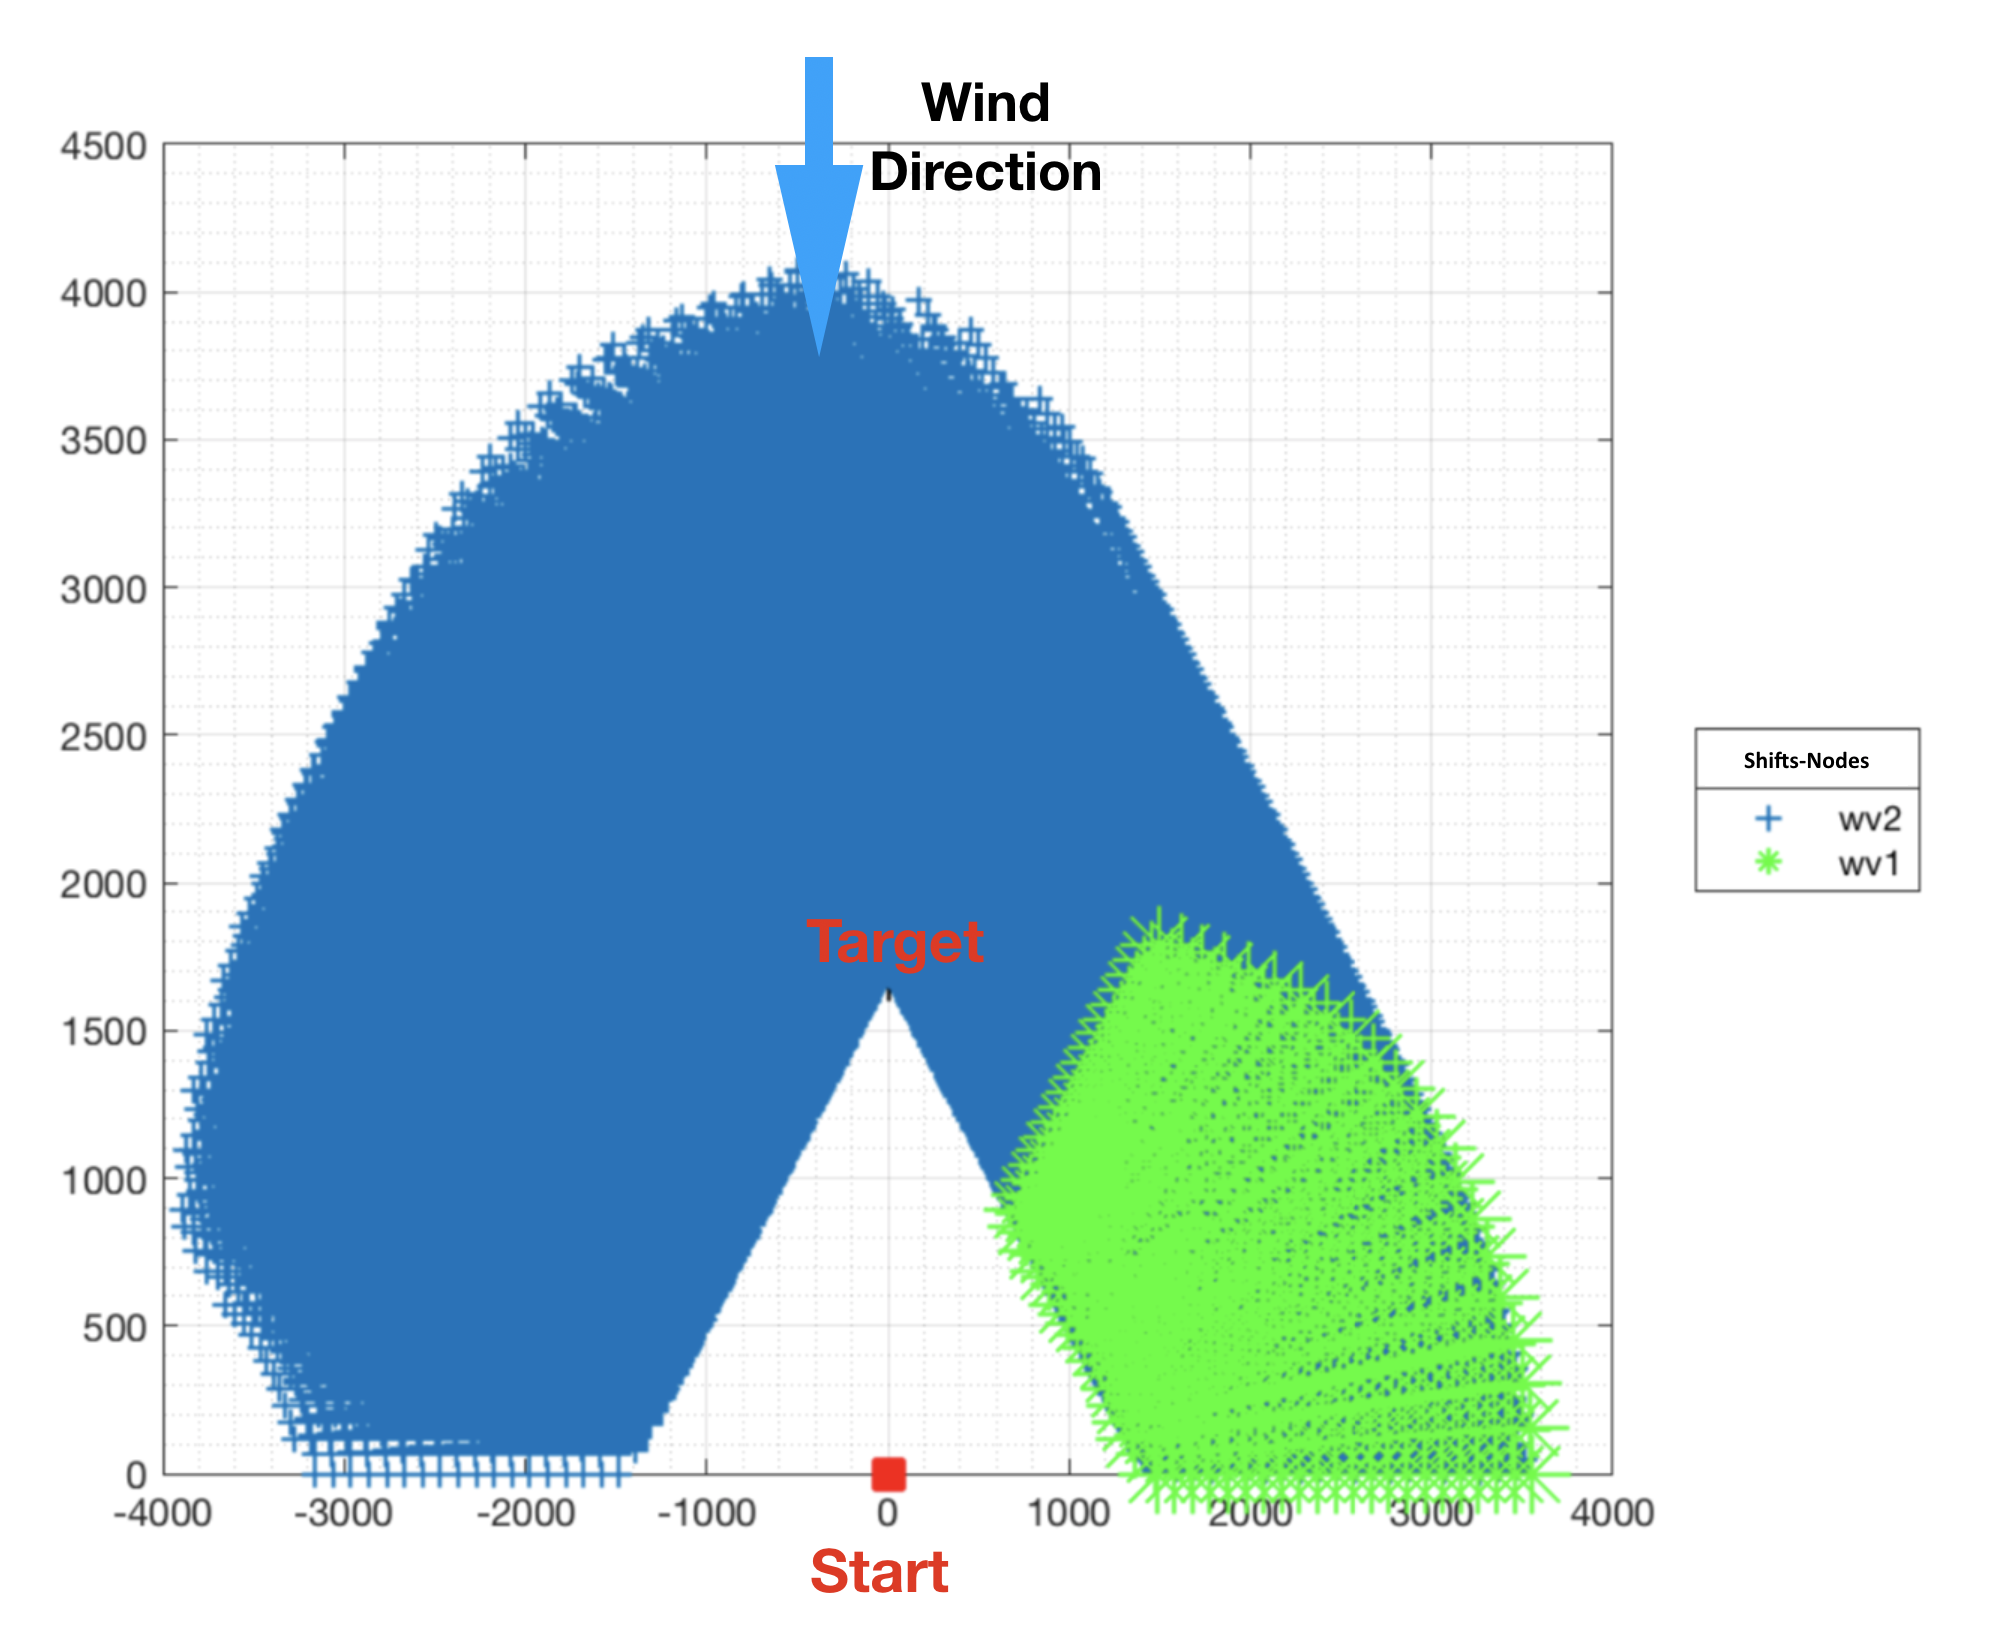
\includegraphics[width=0.28 \linewidth] {images/Nodes_2wv_5deg_5s.png} \label{fig:nodes_2wv_5deg_5s}}
  \hfill
  \subfloat[Sorted Paths from min. to max. time. Only the top 3 are marked in blue.] {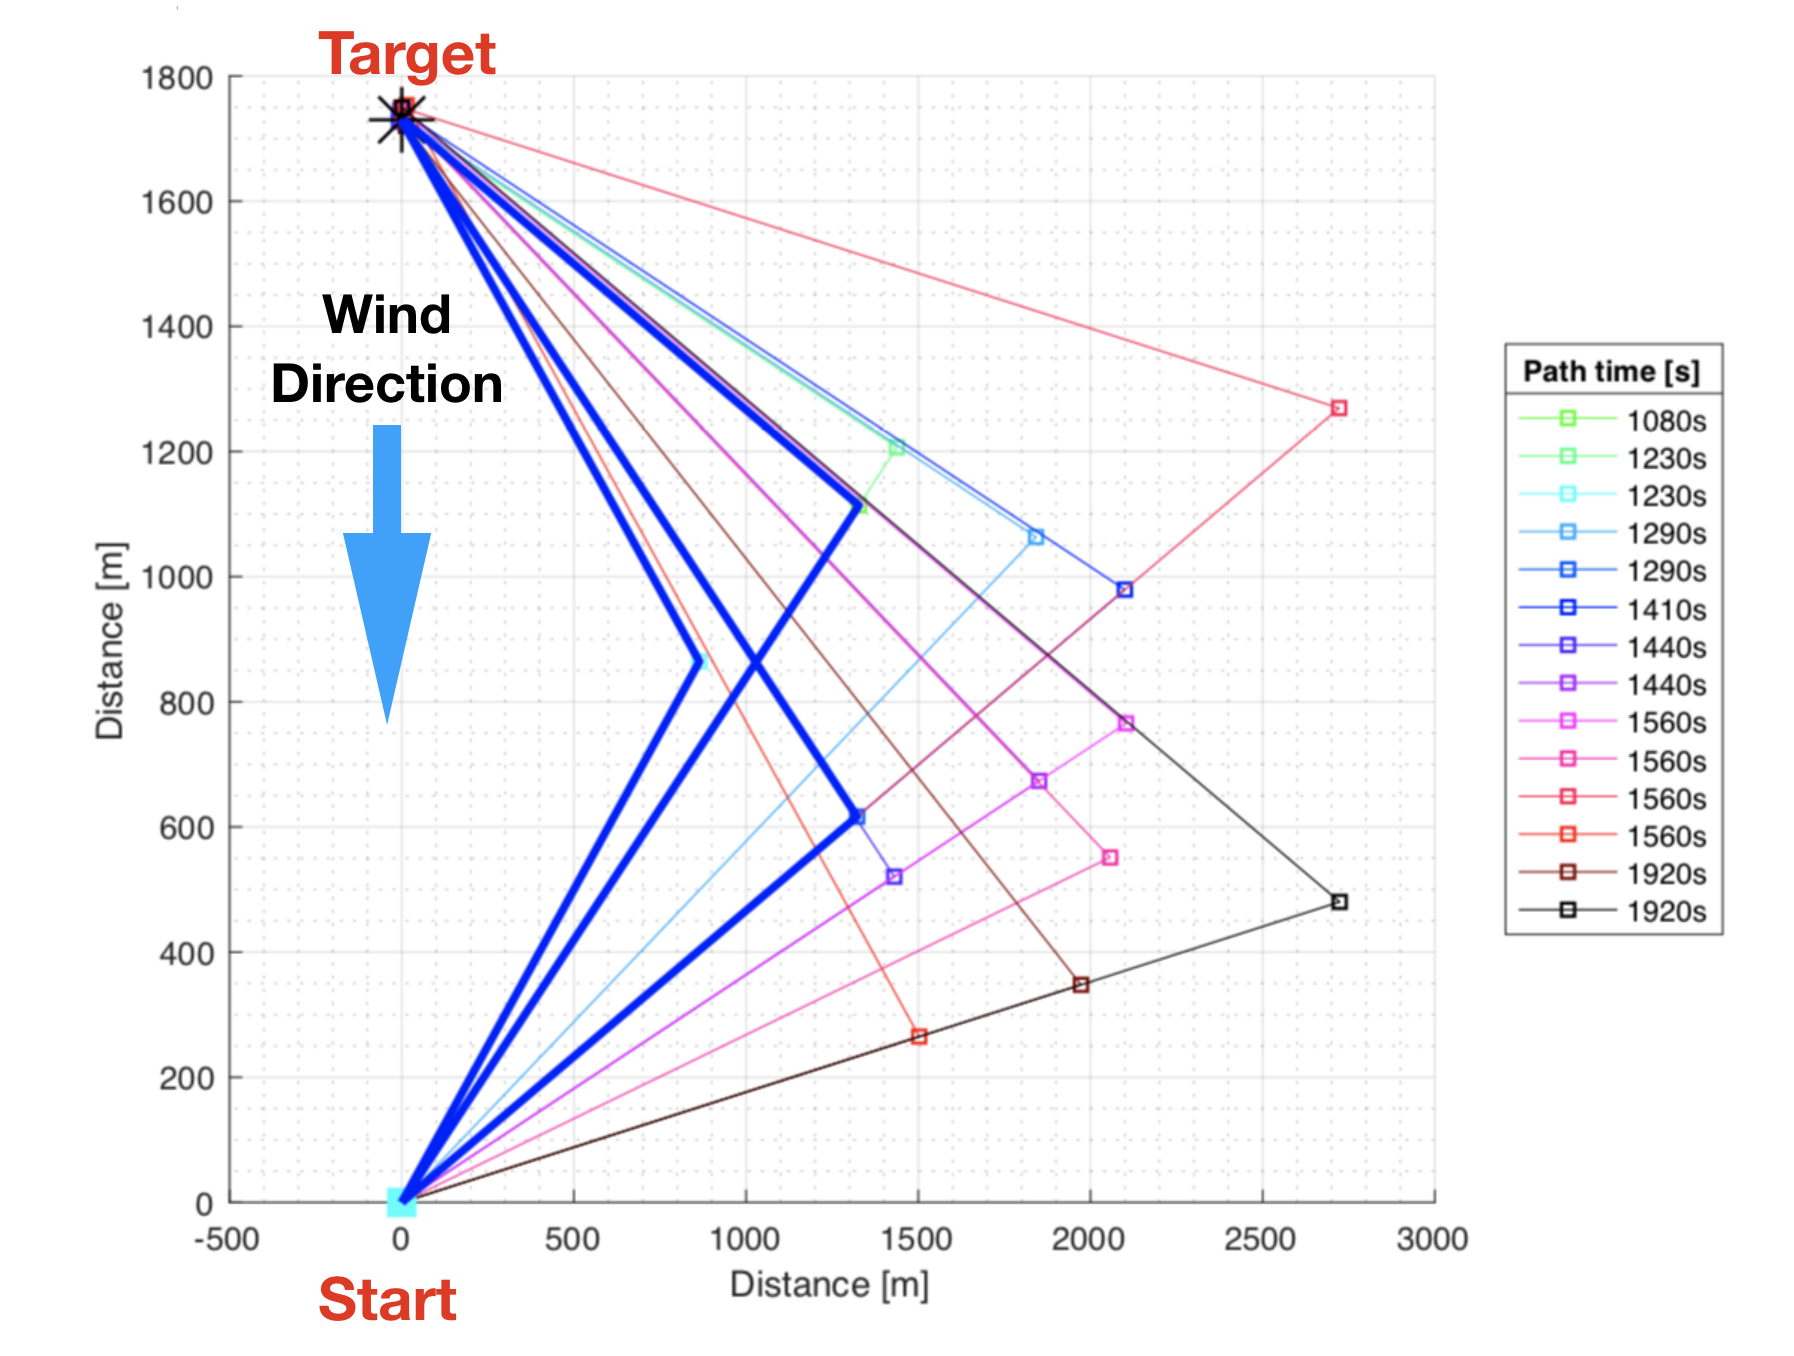
\includegraphics[width=0.32\linewidth]{images/Paths_2wv_5deg_5s.png}\label{fig:Paths_2wv_5deg_5s}}
  \hfill 
  \subfloat[The 3 minimal time paths close-in end at the target.] {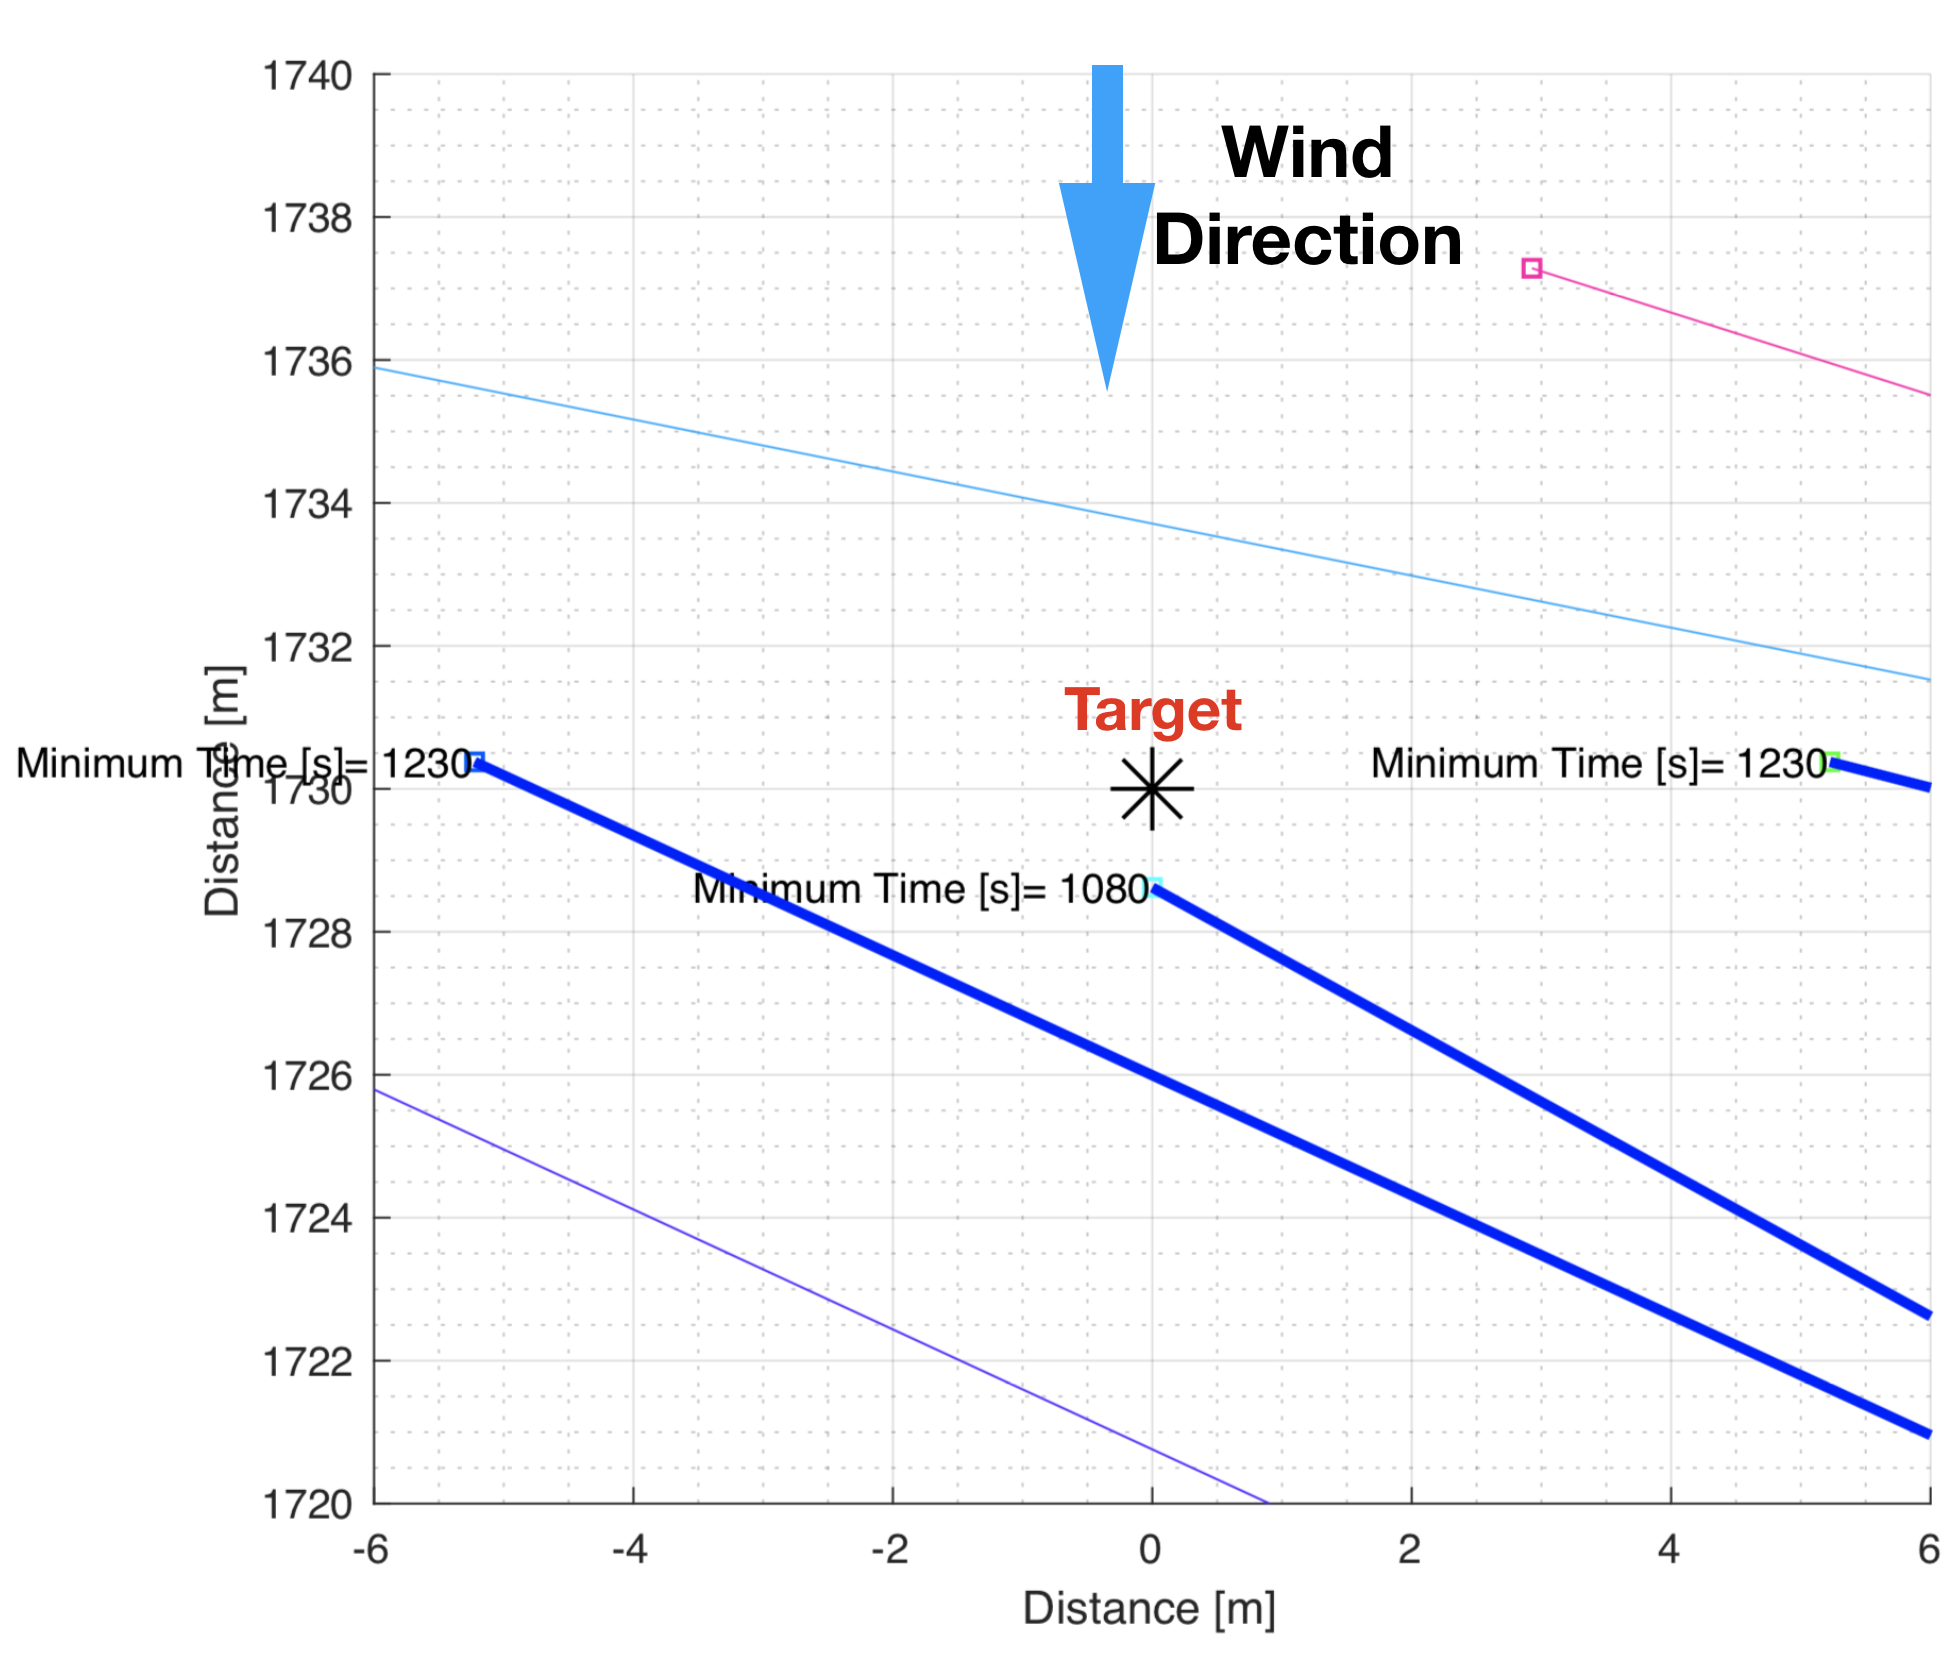
\includegraphics[width=0.32\linewidth] {images/ZoomPaths_2wv_5deg_5s.png} \label{fig:PathsZoom_2wv_5deg_5s}}
  \caption{Nodes and paths generated with one shift in direction with $\Delta t$ =5s and $\Delta \Psi =5\degree$.}
\label{fig:Nodes_Paths_2wv_5deg_5s}
\end{figure}



\newpage
\begin{figure} [hbt!]
  \centering
  \subfloat[Top 5 times using 2 attacks with $\Delta t$ =5s and $\Delta \Psi =1\degree$. All paths have the same time of 1100s] {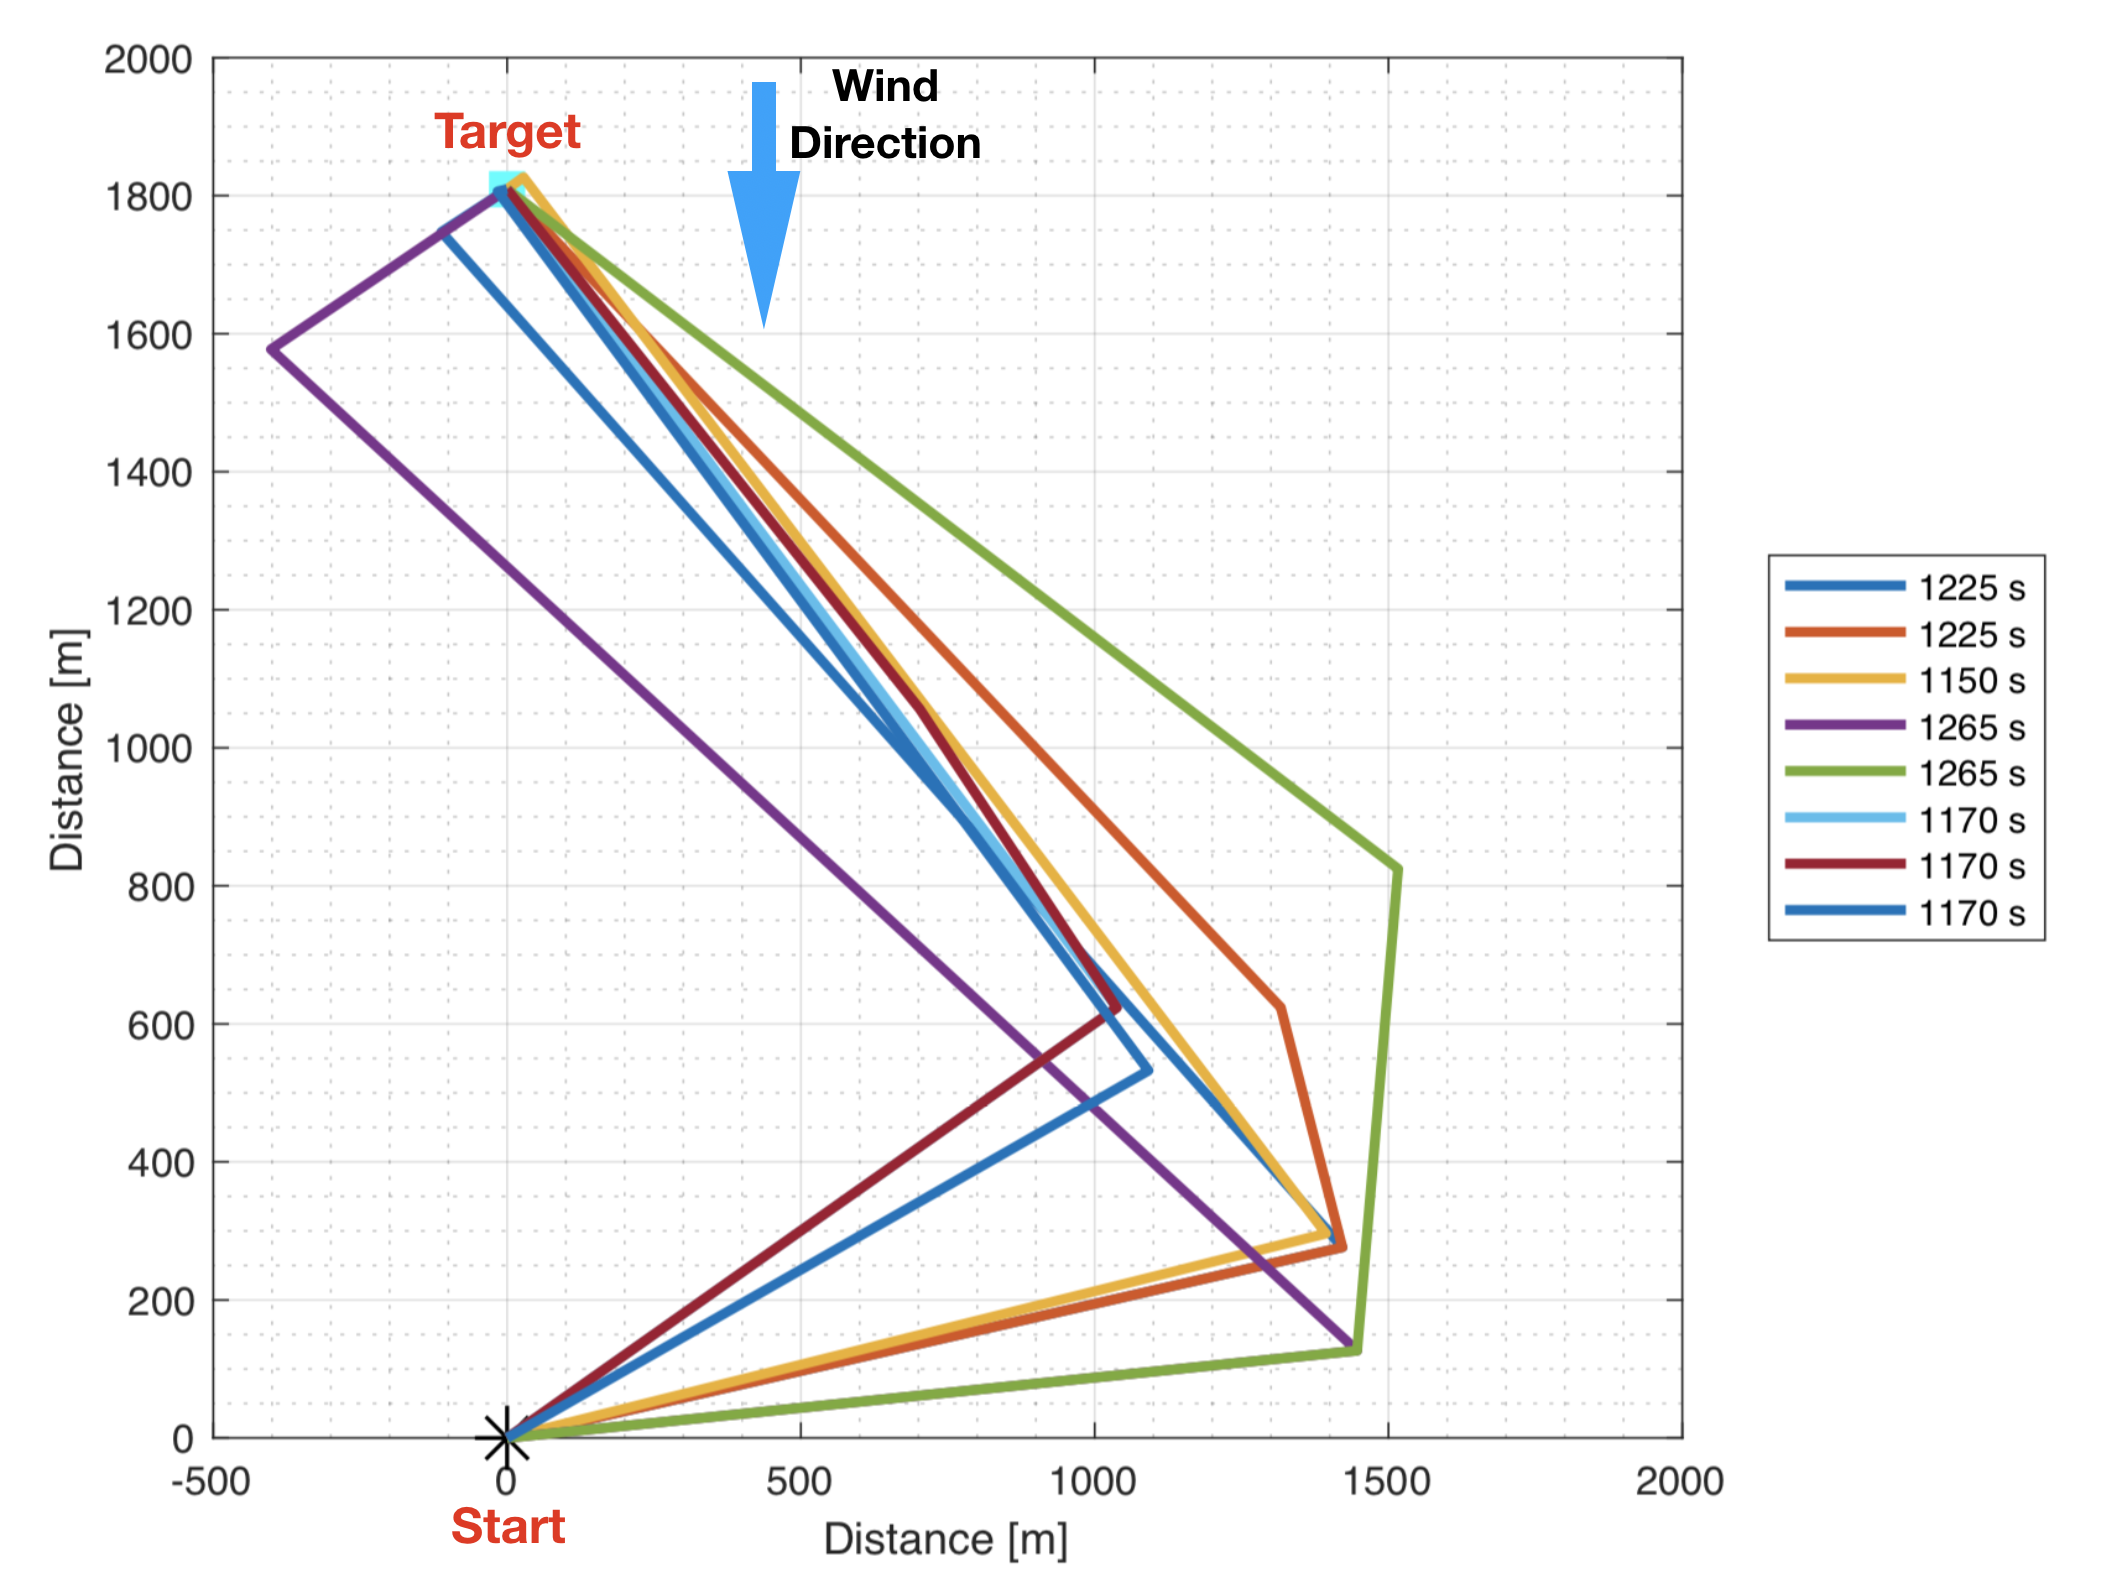
\includegraphics[width=0.45 \linewidth] {images/Paths_3wv_1deg.png} \label{fig:PathsTop_3wv_1deg}}
  \hfill
  \subfloat[Close-up of the top 5 times at the target mark. The ends of paths are within a radius of 3m from the target mark.] {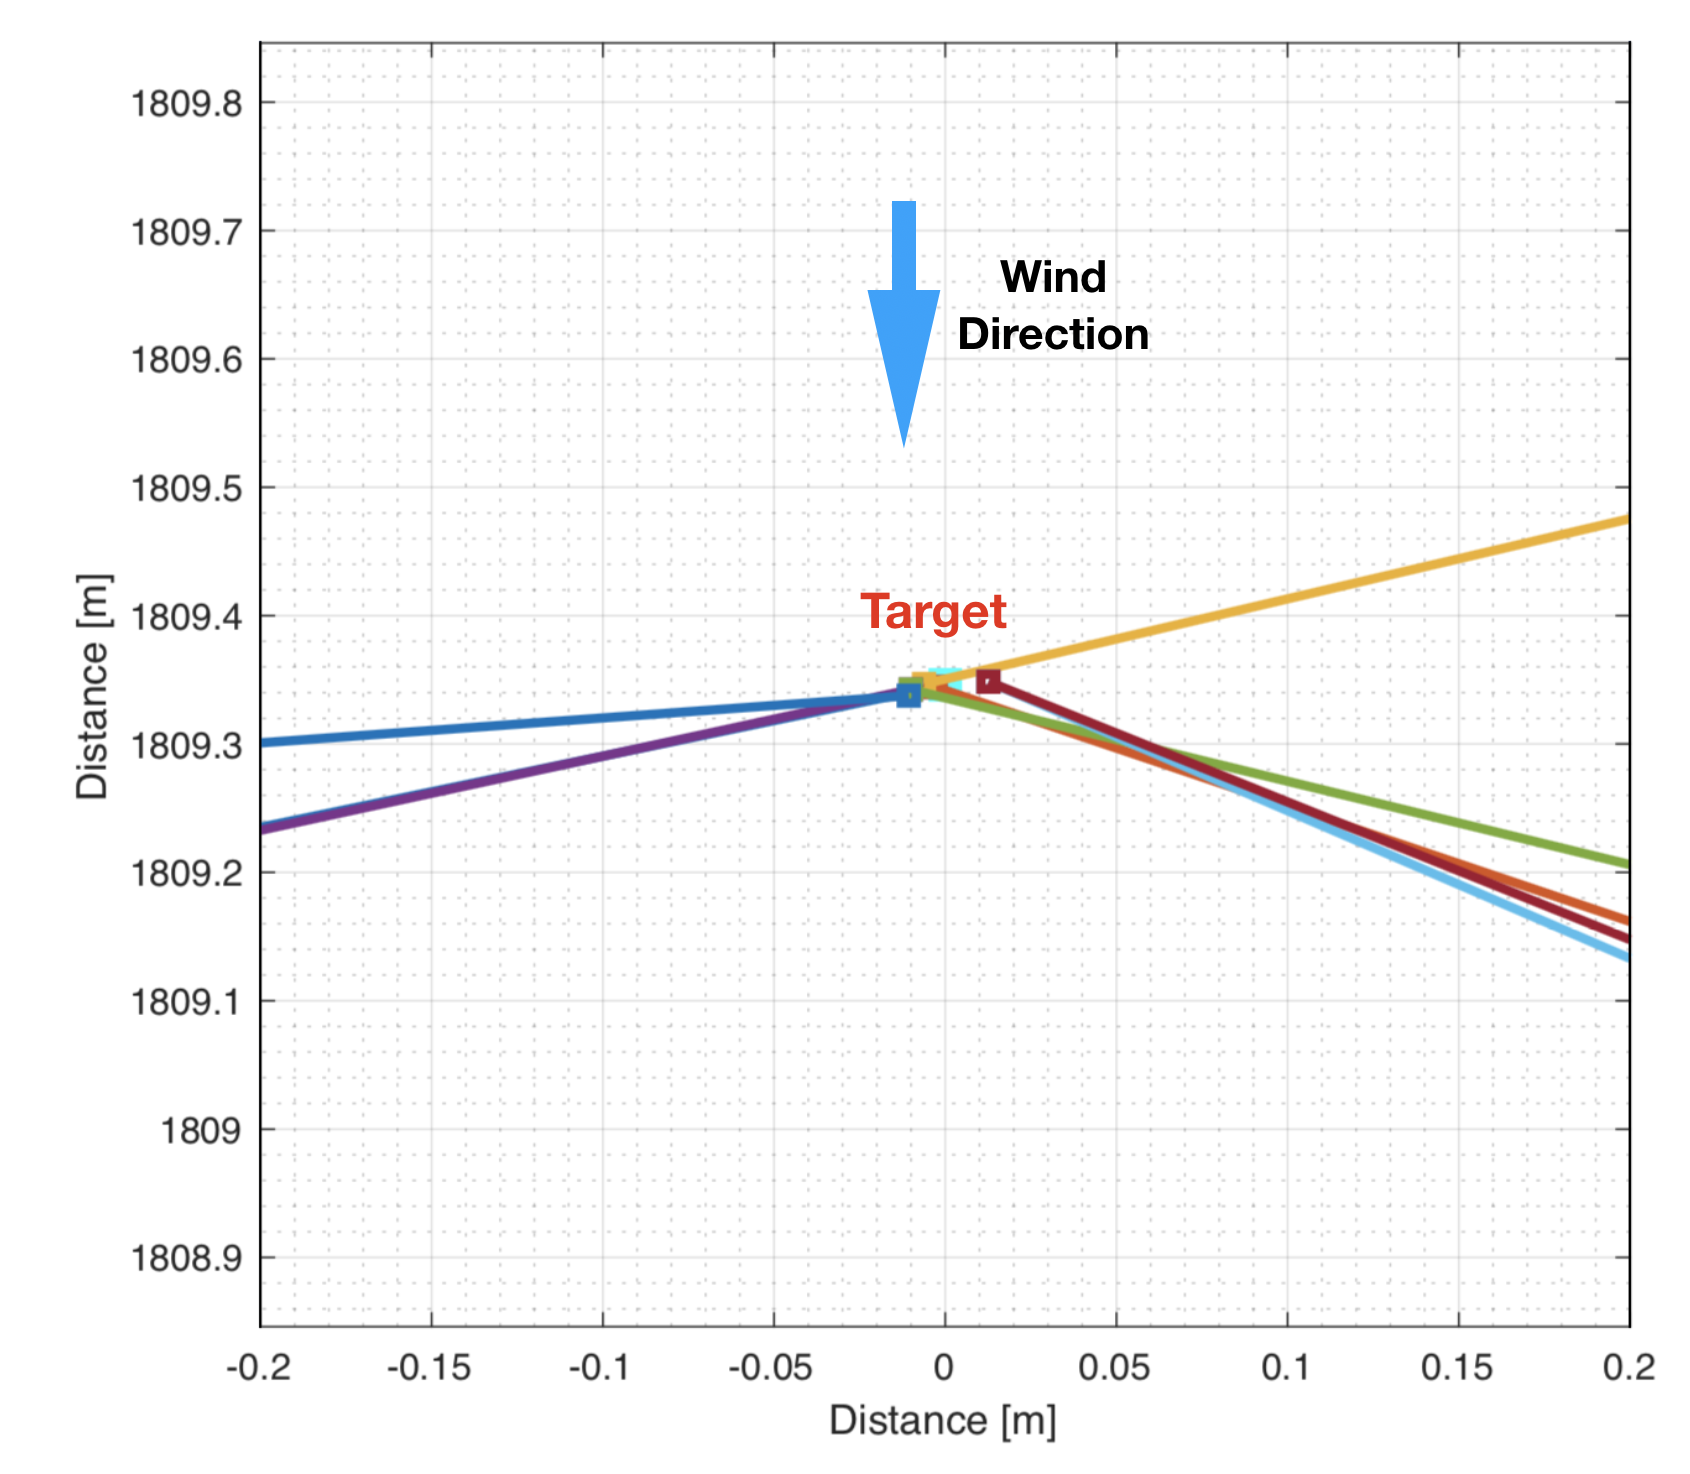
\includegraphics[width=0.4\linewidth]{images/PathsZoom_3wv_1deg.png}\label{fig:PathsZoom_3wv_1deg}}

  \caption{Top 5 time paths and close-up at the target zone with two shifts in direction with $\Delta \Psi =1\degree$, the time of all them is the same and it is 1100 seconds.} %$\Delta t$ =5s and
\label{fig:Paths_3wv_1deg}
\end{figure}
